\documentclass[
	ngerman,
	%twoside,
	BCOR=8mm,
	headings=normal,
	parskip=half,
	headsepline,
	automark,
	listof=totoc,
	bibliography=totoc,
	%,captions=tableabove
	%draft
]{scrreprt}
%
%
%%%%%%%%%%%%%%%%%%%%%%%%%%%%%%%%%%%%%%%%%%%%%%%%%%%%%%%%%%%%%%%%%%%%%%%%%%%%%%%
% Pakete laden
%%%%%%%%%%%%%%%%%%%%%%%%%%%%%%%%%%%%%%%%%%%%%%%%%%%%%%%%%%%%%%%%%%%%%%%%%%%%%%%
%
\usepackage{ifluatex}
\usepackage{babel}
%
\ifluatex
 % LuaLaTeX
 \usepackage{fontspec}
 \usepackage{selnolig}
\else
 % PdfLaTeX
 \usepackage[T1]{fontenc}
 \usepackage{lmodern} % Bei Installation in vscode benötigt: https://tex.stackexchange.com/questions/10706/pdftex-error-font-expansion-auto-expansion-is-only-possible-with-scalable
\fi
%
\usepackage{csquotes}
\usepackage{scrlayer-scrpage}
\usepackage{microtype}
%
%\usepackage{ziffer}% optional
%\usepackage[locale=DE]{siunitx}% optional
%
\usepackage{tikz}
\usepackage{pgfplots}
%
\usepackage[style=authoryear, maxnames=7, backend=biber]{biblatex}
%
\usepackage{amsmath}
\usepackage{amssymb}
%
\usepackage{hyperref}
%
%=== wichtig, dass folgende Pakete NACH hyperref geladen werden ===============
\usepackage{scrhack}% Um Warnung bzgl. \float@addtolists im listings-Paket (s.u.) zu vermeiden
\usepackage{listings}
%
\usepackage[nameinlink]{cleveref}
\usepackage[all]{hypcap}
\usepackage[
	toc,
	symbols,
	acronyms,
]{glossaries}
%
%%%%%%%%%%%%%%%%%%%%%%%%%%%%%%%%%%%%%%%%%%%%%%%%%%%%%%%%%%%%%%%%%%%%%%%%%%%%%%%
% Globale Definitionen
%%%%%%%%%%%%%%%%%%%%%%%%%%%%%%%%%%%%%%%%%%%%%%%%%%%%%%%%%%%%%%%%%%%%%%%%%%%%%%%

%=== pdf Metadaten ============================================================
\hypersetup{
	pdfauthor={Vorname Nachname},
	pdftitle={Vorlage für wissenschaftliche Abschlussarbeiten an der TH Köln},
	pdfsubject={Abschlussarbeit},
	pdfkeywords={
		LaTeX,
		Abschlussarbeit,
		Vorlage,
	},
	bookmarksnumbered=true,
	pdfstartview=FitH,
	hidelinks,
}

%=== Vorwort vor Literatur ====================================================
\defbibnote{mynote}{%
}

%=== Kopf-/Fusszeile definieren ===============================================
\clearpairofpagestyles
\ohead[]{\headmark}
\ofoot[\pagemark]{\pagemark}

%=== Farben definieren ========================================================
\definecolor{THRed}{RGB}{207,24,32}
\definecolor{THOrange}{RGB}{236,101,37}
\definecolor{THPurple}{RGB}{175,54,140}

%=== Einstellungen für cref ===================================================
\newcommand{\crefpairconjunction}{ und~}
\newcommand{\crefrangeconjunction}{ bis~}
\crefname{figure}{Abbildung}{Abbildungen}

%=== Einstellungen für plots ==================================================
\pgfplotsset{
	compat=newest,
	/pgf/number format/.cd,
	dec sep={\text{,}},
	1000 sep={\,},
}

%=== Einstellungen für listings ===============================================
\lstdefinestyle{myLaTeX}{
	basicstyle=\footnotesize\ttfamily,
	language=TeX,
	keywordstyle=\color{blue},
	frame=single,
	backgroundcolor=\color{gray!10},
	tabsize=2,
	morekeywords={
		lstdefinestyle,
		footnotesize,
		ttfamily,
		color,
	},
}

\lstdefinestyle{myBasic}{
	basicstyle=\footnotesize\ttfamily,
	frame=single,
	escapechar={|_},
	backgroundcolor=\color{white},
	keywordstyle=\color{black},
}

\lstset{style=myLaTeX}

%\lstset{language=Python, basicstyle=\small, frame=single, numbers=left, xleftmargin=2em, framexleftmargin=1.5em}
%\renewcommand{\lstlistingname}{Algorithmus}


%=== paar convenience Sachen definieren =======================================
\DeclareMathOperator{\sgn}{sgn}
\newcommand{\vecW}{\ensuremath{\mathbf{w}}}%
\newcommand{\ci}{\ensuremath{\mathrm{i}}}%
%
\newcommand{\tb}{\textbackslash}
%
\newcommand{\comm}[1]{\enquote{\texttt{\tb #1}}}
%
\newcommand{\param}[1]{%
	$\langle$\textrm{\textit{#1}}$\rangle$%
}

%=== Arial als Hauptschriftart ================================================
%\setsansfont{Arial}
%\renewcommand{\familydefault}{\sfdefault}

%
%%%%%%%%%%%%%%%%%%%%%%%%%%%%%%%%%%%%%%%%%%%%%%%%%%%%%%%%%%%%%%%%%%%%%%%%%%%%%%%
% Begriffe für glossaries definieren
%%%%%%%%%%%%%%%%%%%%%%%%%%%%%%%%%%%%%%%%%%%%%%%%%%%%%%%%%%%%%%%%%%%%%%%%%%%%%%%

%=== Glossar ==================================================================
\newglossaryentry{dog}{
	name={Hund},
	description={Behaartes, vierbeiniges Säugetier. Bester Freund des
	Menschen}
}

%=== Abkürzungen ==============================================================
\newacronym{svm}{SVM}{support vector machine}

%=== Symbole ==================================================================
\newglossaryentry{sym:force}{
	name=\ensuremath{\vec{F}},
	description={Kraft, vektorielle Größe},
	type=symbols,
}

%
\makeglossaries
%
\graphicspath{{images/}}
%
\addbibresource{references.bib}

\nocite{*} % listet alle Quellen (auch die nicht zitierten!)
%
%=== für schnelleres kopilieren alle ungeänderten Dateien auskommentieren =====
\includeonly{
	content/Abstract,
	content/Einleitung,
        content/Stand,
        content/Hauptteil,
		content/Code,
}
%
%
%==============================================================================
%
\begin{document}
%
\pdfbookmark[0]{Titelseite}{titel}
\begin{titlepage}
%
\sffamily% Umschalten auf serifenlose Schrift
%
\begin{center}
\begin{tikzpicture}
 \fill[THRed] (0, 0) rectangle (\textwidth/3, 3pt);
 \fill[THOrange] (\textwidth/3, 0) rectangle (2*\textwidth/3, 3pt);
 \fill[THPurple] (2*\textwidth/3, 0) rectangle (\textwidth, 3pt);
\end{tikzpicture}
\end{center}
%
\vfill
%
\begin{huge}
Umsetzbarkeit der Trennung von Percussive und Melodic Frequenzen in einer bereits komprimierten Wav-Datei\\[10mm]
\end{huge}
%
Projektteil der Belegung einer Wahlspezialisierung\newline
%\emph{Master/Bachelor of Arts/Engineering/Laws/Science}\newline
im Studiengang Informatik\newline
an der Fakultät für Informatik und Ingenieurwissenschaften\newline
der Technischen Hochschule Köln
%
\vfill
%
\begin{tabular}{@{}ll}
vorgelegt von: & Lukas Fey, Nicolas Friedmann\\
Matrikel-Nr.:  & 123 456 789, 111 55 463\\
Adresse:       & Auf der Platte.~1\\
               & 51643 Gummersbach\\
               & vorname.nachname@smail.th-koeln.de, nicolas-friedmann@gmx.de\\[5mm]
eingereicht bei:   & Prof. Dr. Lutz Köhler\\
Zweitgutachter*in: & Prof. Dr. Vorname Nachname
\end{tabular}	
%
\\[10mm]
%
Ort, TT.MM.JJJJ%
%
\rmfamily% Umschalten auf Standard-Schrift mit Serifen
%
\end{titlepage}
\cleardoublepage
\pagenumbering{Roman}
\chapter*{Kurzfassung/\emph{Abstract}}
\label{chap:abstract}
%

Diese Arbeit untersucht die Machbarkeit der Trennung perkussiver und harmonischer Frequenzen in einer Wav-Datei.
Im Rahmen des Projekts wird die Fourier-Transformation als Kernmethode zur Signalverarbeitung eingesetzt, um harmonische und perkussive Bestandteile von Audiosignalen zu analysieren und zu extrahieren.
Ergänzend wird auf alternative Methoden wie die Wavelet-Transformation eingegangen, um deren Vor- und Nachteile gegenüber der Fourier-Transformation zu bewerten.

\par

Die praktische Umsetzung erfolgt mit Python und der Bibliothek Librosa.
Die entwickelte Methode ermöglicht es, Audiosignale in getrennte Komponenten zu zerlegen, was vielfältige Anwendungen in der Musikproduktion, Audioanalyse und -restauration eröffnet.
Es wird gezeigt, dass Wav-Dateien aufgrund ihres geringen Informationsverlusts besonders geeignet sind, während MP3-Dateien aufgrund ihrer Verfügbarkeit ein zukünftiges Ziel für Optimierungen darstellen könnten.
Abschließend reflektiert die Arbeit die Limitationen des Ansatzes und gibt einen Ausblick auf mögliche Erweiterungen, einschließlich der Nutzung maschinellen Lernens für komplexere Signaltrennungen.

\cleardoublepage
\pdfbookmark[0]{Inhaltsverzeichnis}{toc}
\tableofcontents
% Tabellenverzeichnis:
% \listoftables
\listoffigures
\printglossary
\printglossary[type=\acronymtype, title={Abkürzungsverzeichnis}]
\printglossary[type=symbols, title={Symbolverzeichnis}]
%
\cleardoublepage
\KOMAoptions{open=right}
\pagenumbering{arabic}
\chapter{Einleitung}
%

Musik ist zu einem Teil des täglichen Labens vieler Menschen geworden. Durch den Konsum und den wirtschaftlichen Ertrag wird an der Produktion und Analyse von Musik geforscht (Quelle?).

\par

Ein Teil der Forschung bezieht sich auf die Trennung einer Wellenform in die unterschiedlichen Funktionen der Frequenzen. Zuvor beinhaltet die Wellenform eine oder mehrere Sinus- und Kosinusfunktionen, die eine neue Funktion bilden. Dies wird sowohl auf audiovisuelle als auch auf visuelle Funktionen angewendet. Beispielsweise kann die Funktion mehrere Instrumente beinhalten, die anhand der Funktion nicht identifizierbar sind. Einer der Algorithmen zur Trennung von Signalen heißt Fourier Transform und wird in diesem Projekt behandelt.

\par

Unter anderem werden Musikinstrumente in Liedern getrennt und einzeln angehört oder wiederverwendet. In diesem Projekt werden zum Einstieg lediglich perkussive aus akkustischen Instrumenten getrennt. Zwischen den jeweiligen Instrumentengruppen wird in \cref{sounds} unterschieden.

%
\section{Relevanz}
%

Es gibt unterschiedliche Kontexte, in denen die Trennung von Audiosignalen zum Einsatz kommt. Häufig ist eine Eingabefunktion als Summe aller Signale schwierig zu analysieren oder weiterzuverarbeiten. Beispielsweise, wenn einzelne Instrumente im Nachhinein bearbeitet werden sollen.

\par

In Zeiten von zunehmend digital produzierter Musik und Verbreitung von Informatik stellt sich die Frage, wie Musiksignale digital aufgebaut sind und wie man mit ihnen arbeiten kann. Im Kontext dieser Arbeit wird die Fourier Transform verwendet, um eine Tondatei in Gruppen von harmonischen und perkussiven Musikinstrumenten zu zerlegen. Dies kann mit weiterer Modifikation verwendet werden, um bestimmte Instrumente zum üben zu trennen oder Hintergrundgeräusche auszublenden.

\par

% Außerdem werden in dem Projekt die Überprüfung der Funktionalität einer Ampel oder das stimmen von Musikinstrumenten in Echtzeit behandelt. Dies sind nur Beispiele dafür, welche Anwendungsfälle es für die Fourier Transform gibt.

(Etwas zu kurz?)

%
\section{Vorgehen}
%

Ohne jegliches Vorwissen, wie die Signale einer Musikdatei gespeichert und von einem Computer interpretiert oder getrennt werden, wird das Projekt durchgeführt. Die Erkenntnisse und notwendiges Hintergrundwissen werden dokumentiert und erklären die Logik und Zusammenhänge der Fourier Transform. Durch die Dokumentation wird anderen Leser:innen ein erstes Verständnis von WAV-Dateien vermittelt auf dem im Anschluss aufgebaut werden kann.

\par

(WAV-Dateien sehr spezifisch: Den Leser:innen wird auch die Funktionalität der FFT und Code etc. vermittelt?)

\par

Das Projekt dokumentiert anschließend die Implementierung eines Algorithmus zur Trennung der harmonischen und perkussiven Tongruppen einer WAV-Datei mittels Fourier Transform, sowie das schreiben auf zwei getrennte WAV-Dateien mittels Inverse Fourier Transform (siehe: \cref{Code}). Dabei wird zuvor behandelte Logik und Hintergrundwissen referenziert und in der Praxis erklärt.
\chapter{Stand der Wissenschaft}
\label{stand_der_wissenschaft}

Die Trennung von Musikinstrumenten ist ein praktischer Anwendungsfall zur Separation von Signalen. Dabei liegen in einer Aufnahme mehrere Signale in Form von einer Funktion vor. In dieser Funktion sind die einzelnen Signale schwierig zu identifizieren.

\par

Bei Vorgehen zur Trennung von Signalen wird die Funktion in eine Abhängigkeit zur Frequenz umgeformt. Anhand der Frequenz können unterschiedliche Signale identifiziert werden. Beispielsweise werden die Frequenzen unterschiedlichen Instrumenten zugeordnet.

\par

Inzwischen wurden mehrere Möglichkeiten zur Transformation einer Funktion in Abhängigkeit zur Zeit in die Abhängigkeit zur Frequenz entdeckt. Diese unterscheiden sich in der Darstellung der Funktion und der Genauigkeit des Ergebnisses.

\par

In diesem Projekt wird die Fourier-Transformation angewendet, die verbreitet und sehr effektiv ist (Quelle?). Es wird überprüft, ob die Implementierung und Anwendung ohne Vorkenntnisse und anspruchsvolle Hardware umsetzbar ist.

% Zusammenfassung der wichtigsten Forschungsergebnisse zu einem bestimmten Thema

% aktueller Stand deines Forschungsfeldes. Du zeigst mit ihm auch auf, an welchem Punkt deine Fragestellung ansetzt.

% https://www.scribbr.de/aufbau-und-gliederung/forschungsstand/
\chapter{Hauptteil}
%

% Bis 3.1 kann weg: wurde nur zum reinkommen geschrieben

Um ein grundlegendes Verständnis für die Analyse von Dateiformaten zu entwickeln wird einem klaren Schema gefolgt. Mit diesem Schema wird sich an der chronologischen Reihenfolge von der Entstehung eines Tons bis zur Verarbeitung im Code orientiert.

%
\begin{enumerate}
    \item Was ist ein Ton
    \item Formen der Musikdarstellung
    \item Vorstellung der Fourier Transform
    \item Alternative Methode zur Fourier Transform
    \item Trennung von Instrumenten im Code
    \item Vorgehen im Projekt (evtl früher)
    \item Wie kann man auf dem Stand aufbauen? (/Wie könnte es weitergehen?)
    \item Fazit
    \begin{enumerate}
        \item Aufwand
        \item Ertrag (z.B. erworbenes Wissen)
    \end{enumerate}
\end{enumerate}
%

Um einen Algorithmus zu implementieren, ist es hilfreich die unterschiedlichen Musikdarstellungen kennenzulernen. Für eine effektive Fourier Transform gibt es Voraussetzungen, die nur von wenigen Musikdarstellungen erfüllt werden.

\par

Außerdem ist es relevant ein Verständnis für die Fourier-Transformation und andere Methoden zu entwickeln, um nachzuvollziehen warum die Fourier Transform geeignet ist. Zudem hilft ein Verständnis bei der Implementierung des Codes.

%
\section{Was ist ein Ton?}
\label{sounds}
%

Töne entstehen durch die Vibration eines Gegenstandes. Diese erzeugen Schallwellen. Das Gehör kann diese Schwingungen der Luft wahrnehmen \parencite{signaltoene}. Der Luftdruck einer Schallwelle wird graphisch als eine Sinus- oder Cosinusfunktion dargestellt.

\begin{figure}[h]
    \centering
    \begin{tikzpicture}[domain=0:10.5]
        \draw[very thin,color=gray] (-0.1,-1.1) grid (10,3.9);
        \draw[->] (-0.2,0) -- (10.5,0) node[right] {$Zeit$}; \draw[->] (0,-1.2) -- (0,4.2) node[above] {$Schalldruck$};
        % \draw[color=blue, samples=150]	plot (\x,{sin(\x r)})	node[right] {$f(x) = \sin x$};
        \draw[color=blue, samples=150]	plot (\x,{sin(pi*\x r)})	node[right] {$\sin x$};
    \end{tikzpicture}
    \caption{Wellenform eines Tons}
    \label{wav_sound}
\end{figure}
\par

Anhand der Wellenform kann die Frequenz eines Tons abgeleitet werden. Diese wird in Hertz (kurz: hz) angegeben. Die Frequenz gibt die Anzahl an Zyklen des Tons pro Sekunde an. Wenn beispielsweise \cref{wav_sound} eine Sekunde darstellt, entspricht die Frequenz 53hz.

Diese Vibration kann durch unterschiedliche Gegenstände erzeugt werden. Dazu zählen Becken eines Schlagzeugs, Saiten eines Kontrabasses oder die Stimmbänder. In diesem Projekt werden die Perkussionsinstrumente von den restlichen Instrumenten einer Wav-Datei getrennt. 

\par

Akkustische Instrumente erzeugen einen Ton indem Menschen Kraft auf sie ausüben. Sie benötigen keinen Strom, keine Verstärkung und keinen Computerprozessor, um einen Ton zu erzeugen und sind die ältesten Instrumente. Sie können in perkussive und harmonische Instrumente unterteilt werden. Perkussive Instrumente werden geschlagen, geschütttelt oder geschabt und sind eine spezielle Form der akkustischen Instrumente. Die übrigen akkustischen Instrumente sind harmonisch \parencite{acoustic_electric_digital_instruments}.

\par

Neben akkustischen existieren noch elektrische und digitale Instrumente. Sie benötigen entweder Elektrizität oder einen Computerprozessor, um wie vorgesehen zu funktionieren. Allerdings werden sie in diesem Projekt nicht behandelt.

%
\section{Formen der Musikdarstellungen}
%

Musik kann unterschiedlich dargestellt werden. Je nach Bedarf, wird eine andere Form der Musikdarstellung benötigt. Es werden Musiknoten, symbolische Darstellungen und Audiodarstellungen verwendet. Es ist eine formale Sprache, die vorgibt wie ein Musikstück gespielt wird \parencite{sheet_music_representations}. Bei symbolischen Darstellungen werden eindeutige Entitäten definiert, die von einem Computer übersetzt werden. Beispielsweise wird der Musical Instrument Digital Interface (kurz: MIDI) Standard verwendet, um Informationen eines gespielten Tons möglichgst detailliert zu speichern und abzurufen.

\par

Eine weitere Form der Darstellung, ist die Audiodarstellung. In diesen Darstellungen werden alle Informationen der Töne als Audiosignale digital gespeichert und geteilt. Es werden die Schallwellen eines Tons (siehe \cref{sounds}) aufgenommen und digital als eine Wellenform gespeichert, die an der Schallwelle orientiert ist. Dazu gehören auch das Timing, die Intensität, die Lautstärke, die Länge des Tons und vieles mehr. Es werden nicht die einzelnen Töne und Noten gespeichert, sondern die Frequenzen während der Aufnahme in Abhängigkeit zur Zeit. Die Audiodatei kann auch Nebengeräusche oder weitere Instrumente beihalten (\cite{fundamentals_of_music_processing}, S. 1ff).

\subsection{Einordnung in den Projektkontext}

Die digitale Darstellung macht es schwieriger unterschiedliche Audiosignale zu trennen und die ursprünglichen Töne wieder herzustellen. Die verbreitetste Form der Audiodarstellung ist MP3 \parencite{mp3_most_popular}. In diesem Projekt werden jedoch Wav(einheitlich?)-Dateien behandelt. Die Unterschiede, sowie Vor- und Nachteile der Audiodarstellungen werden in \cref{audio_representations} behandelt \parencite{fundamentals_of_music_processing}.

%
\section{Aufbau einer Audiodatei/ Music Representation}
%

Für die Aufnahme von Audiosignalen werden analoge Signale in eine digitale Form von Schall umgewandelt. Die analoge Signaldarstellung basiert auf kontinuierliche und konstante Spannungsschwankungen, die den verursachten Luftdruckschwankungen entsprechen \parencite{digital_representation}. In der digitalen Form werden die Spannungsschwankungen als Bitstreams gespeichert und je nach Audio-Format komprimiert.

%
\subsection{Durchführung der Komprimierung}
\label{compression}
%

Die Komprimierung von Audiodateien wird meistens verwendet, um mehr Musik auf einem Datenträger speichern zu können \parencite{what_is_audio_compression}. Um eine Aufnahme zu komprimieren wird diese in eine Samplingrate (auch: Abtastrate) und eine Quantisierungsschrittweite reduziert.

\par

%
\textbf{Samplingrate}
%

Die Samplingrate definiert die Anzahl von gespeicherten Signalen pro Sekunde. Dies reduziert die benötigten gespeicherten Daten von einer durchgängigen Aufnahme auf mehrere Blöcke. Beispielsweise hat eine CD Aufnahme eine Samplingrate von 44.100 Samples pro Sekunde (kurz: 44.1 kHz), das heißt es werden 44.100 Soundsignale pro Sekunde gespeichert, dessen Übergänge kaum wahrnehmbar sind, jedoch bereits zu einem deutlichen Reduzierung des Speicherbedarfs führen.

%
\textbf{Quantisierungsschrittweite}
%

Die Quantisierungsschrittweite beschreibt die Auflösung, mit der jedes Sample komprimiert wird. Die möglichen Werte eines Samples sind kontinuierlich und könnten theoretisch unendlich viele Dezimalstellen haben. Durch die Quantisierungsschrittweite werden diese Werte jedoch auf eine festgelegte Anzahl möglicher diskreter Werte reduziert, wodurch der Unterschied zwischen den Werten bestimmt wird. Bei CDs wird beispielsweise eine 16-Bit-Codierung gewählt, die 65.536 mögliche Werte definiert.

%
\begin{figure}[h]
    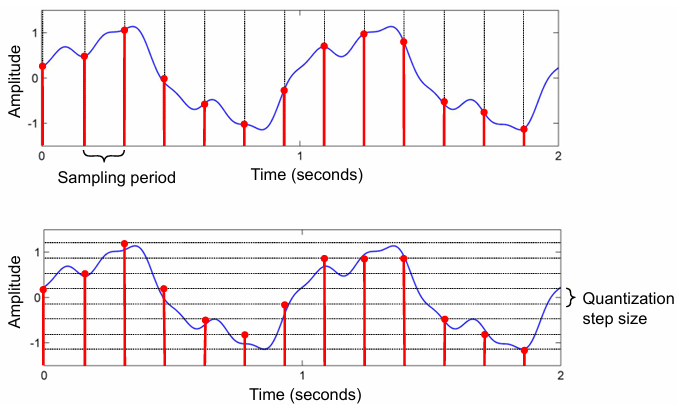
\includegraphics[width=0.5\textwidth]{images/Samplingrate_Quantisierungsgröße.PNG}
    \caption{Unterteilung in Samplingrate (oben) und Quantisierungsschrittweite (unten)}
    \label{fig:samplingrate}
\end{figure}
% Music Processing S.61
%

%
\subsection{Waveform Audio File Format}
%

Das Waveform Audio File Format (kurz: WAV) speichert Audioaufnahmen unkomprimiert \parencite{what_is_a_wav_file}. Der Begriff leitet sich \enquote{vom englischen Wort \enquote{wave}} für Schallwelle ab \parencite{wav}. Für die in diesem Projekt behandelte Fourier Transform sind insbesondere die \enquote{Abtastrate fs des Messsystems} und die Quantisierungsschrittweite (siehe \cref{compression}) entscheidend  \parencite{FFT_grundlagen}. Aufgrund der unkomprimierten Speicherung (und der damit verbundenen hohen Abtastrate und Quantisierungsschrittweite) lässt sich eine klare Trennung von Tonspuren ermöglichen (Referenz?).


%
\subsection{Andere Formen von Audio-Dateien}
\label{audio_representations}
%

%
\begin{itemize}
    \item MP3
    \item WMA
    \item AAC
    \item OGG
    \item FLAC
    \item RM
\end{itemize}
%

\parencite{audioformate_im_überblick}

%
\section{Trennung einer Tonspur in verschiedene Instrumente}
%

Eine Aufnahme speichert das aufgenommene Signal in Abhängigkeit zur Zeit. Jedes eingehende Signal verfügt über Schwingungen in Form von einer Wellenform. Bei einer Aufnahme vermischen sich die verschiedenen Signale zu einer gemeinsamen Wellenform und sind daher schwierig voneinander zu unterscheiden, beispielsweise bei Hintergrundgeräuschen oder der gleichzeitigen Aufnahme mehrerer Musikinstrumente.

\par

Die Trennung von Instrumenten innerhalb einer Tonspur ist ein Thema, das in Forschung und Bildung intensiv behandelt wird (Quelle?). Die am häufigsten verwendete Methode ist die Fourier Transform (Quelle?), die es ermöglicht, ein Signal in seine Frequenzkomponenten zu zerlegen.

\par

Neben der Fourier Transform werden auch andere Ansätze wie die WaveletbTransform, die Short-Time Fourier Transform (kurz: STFT), sowie statistische Verfahren wie die Blind Source Separation (BSS) und die Independent Component Analysis (ICA) eingesetzt. Darüber hinaus finden moderne Verfahren des maschinellen Lernens, insbesondere neuronale Netzwerke, zunehmend Anwendung in der Trennung von Audiosignalen.

%
\subsection{Fourier Transform}
%

Die Fourier Transform ist ein Algorithmus der die Darstellung einer Tondatei verändert. Ursprünglich liegt die Audiospur mit einer Kombination aus unterschiedlichen Frequenzen in Abhängigkeit zur Zeit vor. In dieser Darstellung sind die unterschiedlichen Signale schwierig zu trennen und werden von der Fourier Transform transformiert.

\par

%
\subsubsection{Entwicklung der Fourier Transform}
%

Die Fourier Transform ist eine Verallgemeinerung der Fourierreihen. Diese Reihen können stetige oder stückweise stetige Funktionen in eine Summe von Sinus- und Kosinusfunktionen zerlegen. Bereits im 18. Jahrhundert wurden Fourierreihen für spezifische Funktionen entdeckt. 1822 stellte Joseph Fourier die Hypothese auf, dass sich jede Funktion als Summe solcher Reihen darstellen lässt. Erst im 20. Jahrhundert wurden Fourierreihen auch für andere stetige oder stückweise stetige Funktionen formal bewiesen. Dank der Vollständigkeiten der Funktionenreihe lässt sich die Fourier Transform auf eine Vielzahl von Funktionen anwenden, einschließlich periodischer und nicht-periodischer Funktionen, und erhielt ihren Namen zu Ehren von Fourier.

\par

\subsubsection{Durchführung der Transformation}

Die Fourier Transform ist ein mathematisches Verfahren, bei dem ein Signal aus dem Zeitbereich in den Frequenzbereich transformiert wird. Die Transformation ermöglicht es, beliebige periodische und stückweise stetige Funktionen als Summe von Sinus- und Kosinuswellen unterschiedlicher Frequenzen darzustellen.

\par

%  - Vergleichsschwingungen
 
\par

In der neuen Darstellung werden die Frequenzen der Funktion unabhängig von der zeitlichen Komponente wiedergegeben. Unterschiedliche Frequenzen können unterschiedlichen Signalen zugeordnet werden. Die frequentielle Darstellung gibt an welche Signale in welchen Frequenzen Teil der Funktion sind, allerdings nicht wann. Daher wird die Darstellung wieder umgeformt in die zeitliche Abhängigkeit.

\par

Das Signal oder die Signale, die von der Tonspur getrennt werden, können in der frequentiellen Darstellung identifiziert werden. Anschließend werden diese von den übrigen Signalen getrennt und zurück in die ursprüngliche Darstellung transformiert (Inverse Fourier Transform). Damit erhält man eine neue Tondatei, die ausschließlich aus den benötigten Signalen besteht.

% \subsubsection{Parameter der Transformation}

%  - Probleme:
%     - Rechenaufwand/ Dauer

% In \cref{compression} wurden die relevanten Parameter wie Samplingrate und Quantisierungsschrittweite behandelt, die für die Durchführbarkeit der Transformation entscheidend sind. Zudem können verschiedene Komponenten der Transformation konfiguriert bzw. parametrisiert werden.

% \par

% %
% \textbf{Blocklänge (/engl.?)}
% %

% Ein wesentlicher Parameter für die Durchführung der Fourier Transform ist die Blocklänge (kurz: BL), welche die Anzahl der Samples festlegt, die in der Fourier Transform analysiert werden.

% \par

% Umso länger die BL, desto präziser ist das Ergebnis der Transformation. Dies erhöht jedoch auch den Rechenaufwand und die Dauer der Transformation. In einigen Anwendungsszenarien erfordert dies eine Abwägung zwischen Verarbeitungsdauer und Genauigkeit, beispielsweise in einer App zum Stimmen von Musikinstrumenten oder zum Erkennen der gespielten Töne (Quelle?).

\par

\subsubsection{Durchführung am Beispiel einer Musiknote}

In diesem Beispiel (aus \cite{fundamentals_of_music_processing}, S.40f) wird eine Note auf einem Piano gespielt und durch die Transformation in eine frequentielle Darstellung der gespielte Ton erkannt.

\par

% Die Aufnahme des Tons ist in \cref{fig:fourier}(a) zu erkennen. Für die Transformation wird ein Ausschnitt von 10ms verwendet. Das entspricht der Blocklänge und reduziert den Rechenaufwand (referenzieren?).

Die Aufnahme des Tons ist in \cref{fig:fourier}(a) zu erkennen. Für die Transformation wird ein Ausschnitt von 10ms verwendet, um den Rechenaufwand zu reduzieren.

%
\begin{figure}[h]
    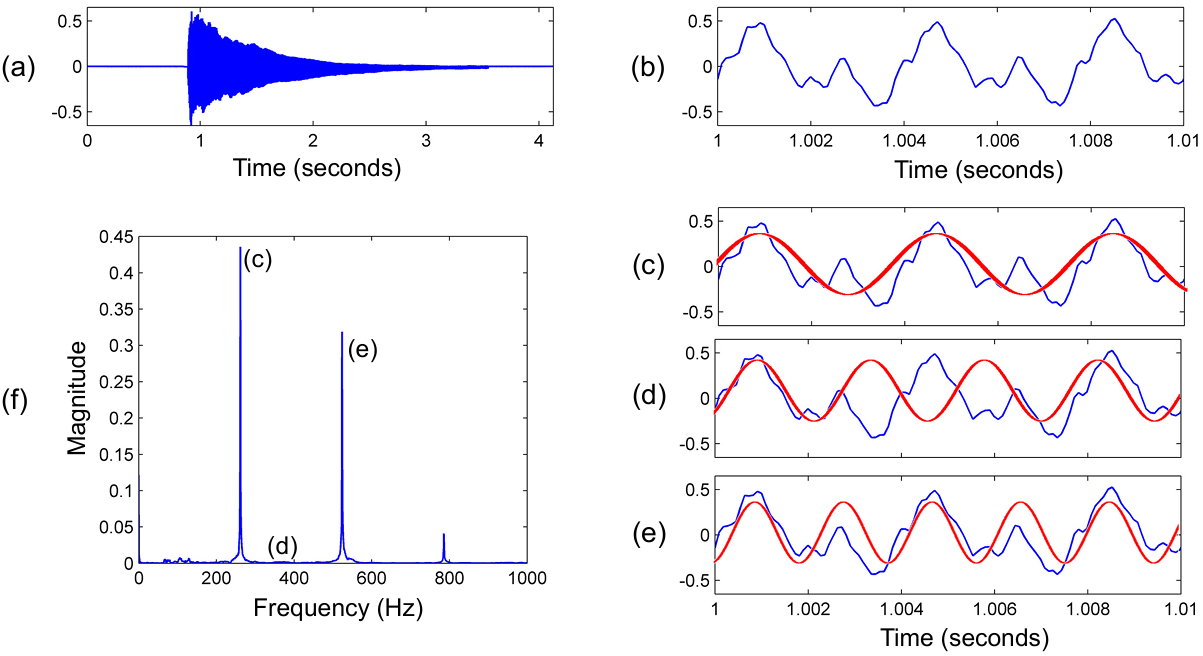
\includegraphics[width=1\textwidth]{images/Fourier_math.PNG}
    \caption{Note C4 in unterschiedlichen Darstellungen (\cite{fundamentals_of_music_processing}, S. 41)}
    \label{fig:fourier}
    \end{figure}
    % Music Processing S.41
    %
\par

Anschließend werden unterschiedliche Vergleichsfunktion für die jeweiligen Frequenzen mit dem Ausschnitt der Tonspur verglichen. Die Ähnlichkeiten der jeweiligen Frequenzen werden in (f) wiedergegeben.

\par

In \cref{fig:fourier}(c) ist die Übereinstimmung für die Frequenz w = 262 Hz besonders hoch. Daraus folgt in (f) bei ungefähr 262 der höchste Wert. Die Höhe des Wertes wird in der Variable dw angegeben.

% w = ω

\par

Die Frequenz 262 entspricht der Note C4. Darüberhinaus wird bei einer Frequenz von 523 (siehe \cref{fig:fourier}(e)) eine hohe Übereinstimmung erkannt. Dies entspricht ungefähr der Frequenz des zweiten Teils der Note C4 (zweiter Teil?).

%
\textbf{Nachteile}
%
    
Die Fourier Transform ermöglicht es je nach Bedarf zwischen der zeitlichen oder der sequentiellen Darstellung zu wechseln. Allerdings ist bei der Fourier Transform der Wechsel zwischen den Darstellung notwendig und es wird entweder die zeitliche oder die frequentielle Komponente ignoriert. Bei der Anwendung der Fourier Transform gibt es keine Darstellung die beide Komponenten kombiniert.

    - Darstellung (nie Zeit und Frequenz)

(Noch unklar wie unterschiedliche Instrumente vorliegen, aber analoge Instrumente sollten in Sinusfunktion vorliegen und erkennbar sein)
(Lukas: Alle Instrumente bzw Töne der Instrumente liegen als Sinuswellen vor)

%
\subsection{Wavelet Transform}
\label{wavelet-transformation}
%

Die Wavelet Transform ist ein Verfahren, das eine zeitliche Darstellung einer Funktion in eine dreidimensionale Darstellung in Abhhängigkeit von Zeit und Frequenz überführt. Dabei werden sogenannte Wavelets - spezielle Wellenfunktionen - mit der ursprünglichen Funktion verglichen, um Übereinstimmungen zu finden. Der Begriff \enquote{Wavelet} stammt aus dem Französischen und bedeutet \enquote{kleine Welle} oder \enquote{Wellchen}.

\par

Im Gegensatz zur ursprünglichen Funktion haben die Wavelets eine endliche Fläche (auch: finite energy), was sie begrenzt und lokalisiert. Eine weitere Bedingung für Wavelets ist, dass ihr Integral gleich null ergibt, d.h., dass die Fläche über und unter der X-Achse gleich groß ist (Admissibility condition). 

\par

Jedes Wavelet wird durch die Parameter m und b ergänzt:

%
\begin{itemize}
    \item[m:] Bestimmt die Frequenz des Wavelets
    \item[b:] Bestimmt den Zeitpunkt des Wavelets
\end{itemize}
%

Zudem besitzt das Wavelet einen realen und einen imaginären Teil. Durch die Berücksichtigung des imaginären Teils entsteht eine dreidimensionale Darstellung des Signals. Bei der Wavelet Transform wird sowohl der reale als auch der imaginäre Teil des Wavelets mit der Funktion korreliert (Mathematik: Korrelation), um die Ähnlichkeit der Funktion und des Wavelets zu berechnen. Diese Ähnlichkeit wird für jedes m und b ermittelt und in einem dreidimensionalen Ausgabe-Graphen in Abhängigkeit von der Zeit dargestellt. Dadurch ergibt sich eine Darstellung des Signals in Bezug auf Zeit und Frequenz.

\par

Ein Anwendungsfall ist die Überprüfung von Ampelleuchten. Während die Fourier-Transformation die verschiedenen Frequenzen der Farben Grün, Gelb und Rot erkennen kann, um festzustellen, ob die Lampen leuchten, erlaubt die Wavelet Transform zusätzlich die Angabe, ob die Lichter zu den richtigen Zeitpunkten aufleuchten \parencite{wavelets}.

%
 - verwendet spezialisierte Funktionen: Wavelets
 - aus französisch Wellchen/ kleine Welle
 - Familie an Funktionen
   - jede für spezielle Anwendung
 - Integral unter und über X-Achse gleichgroß
   - Admissibility condition
 - endliche Fläche
   - finite energy
   - lokalisiert in Zeit

%
\subsection{Wahl der Fourier Transform}
%

Für die Trennug der Instrumente einer Wav-Datei wurde die Fourier Transform gewählt, trotz einiger Alternativen. Die Fourier Transform ist eins der meistverwendeten Werkzeuge der Signalverarbeitung (Müller Kap. 2). Der größte Nachteil der Fourier Transform ist, dass nicht gleichzeitig die Zeit und die Frequenz Domäne dargestellt werden können. Allerdings reicht dies bei der Trennung von Musikinstrumenten, da die Darstellung zum Schluss wieder in die zeitliche Domäne umgeformt werden soll, um das Ergebnis in eine Wav-Datei zu überführen. Außerdem verliert die Fourier Transform wenig Informationen durch die klare Trennung von zeitlicher und frequentieller Darstellung (https://academic.oup.com/jmammal/article-abstract/81/4/927/2372896). Allerdings ist die Fourier Transform bei größeren Dateien aufwändiger und fehleranfälliger, falls die ganze Datei transformiert wird (auch zu Nachteile?). Jedoch wird diese Limitierung durch die Verwendung der Short-Time Fourier Transform reduziert (https://www.sciencedirect.com/science/article/abs/pii/S1746809416301859: 6.1.3.1).

%
\subsection{Short-Time Fourier Transform}
%

Die Short-Time Fourier Transform (auch: STFT) basiert auf der Fourier Transform, dessen Nachteile zunehmender Aufwand und fehleranfälligkeit bei der Transformation größerer Dateien beihaltet (siehe: Nachteile oder Wahl?).

\par

Stattdessen teilt die Short Time Fourier Transform eine Datei in mehrere kleine Pakete, deren Transformation effizienter und effektiver durchgeführt werden können. Anschließend werden die Übergäge der Pakete geglättet (Wortwahl?), um unregelmäßigkeiten (groß?) zu vermeiden. In \cref{stft_code} wird die praktische Umsetzung mittels Programmcode dargestellt und die Funktionalität erläutert.
\chapter{Code}
\label{Code}

In diesem Abschnitt wird der Python-Code zur Extraktion von harmonischen und perkussiven Komponenten aus Audiodateien unter Verwendung der Bibliothek \texttt{librosa} detailliert erklärt.

\section{Beschreibung des Codes}

Der Code beginnt mit dem Importieren der benötigten Bibliotheken, um Audio zu laden, zu verarbeiten und in neue Dateien zu schreiben:

\begin{lstlisting}[language=Python, caption={Bibliotheken importieren}]
import os
import librosa
import soundfile as sf
import numpy as np
\end{lstlisting}

Hierbei ist \texttt{librosa} die zentrale Bibliothek zur Verarbeitung von Audiodaten, während \texttt{soundfile} für das Schreiben der resultierenden Audiodateien verwendet wird. 

\section{Hauptfunktion: \texttt{harmonic\_extraction}}

Die Hauptfunktion des Codes ist \texttt{harmonic\_extraction}, die einen Dateipfad für die Audiodatei und einen Namen für die Ausgabedatei als Parameter erhält. 

\begin{lstlisting}[language=Python, caption={Die Funktion \texttt{harmonic\_extraction}}]
def harmonic_extraction(audio_path, output_filename):
    y, sr = librosa.load(audio_path)
    
    y_harmonic, y_percussive = librosa.effects.hpss(y)
\end{lstlisting}

Die Funktion beginnt mit dem Laden der Audiodatei. Die Methode \texttt{librosa.load} lädt die Datei und gibt das Audiosignal \texttt{y} und die Sampling-Rate \texttt{sr} zurück. Der nächste Schritt ist die Verwendung der Harmonic-Percussive Source Separation (HPSS) Funktion \texttt{librosa.effects.hpss(y)}, die das Audiosignal in harmonische und perkussive Komponenten zerlegt. Dies geschieht mithilfe der Fourier-Transformation.

\section{Speichern der Ergebnisse}

Nach der Zerlegung speichert der Code die beiden Komponenten in separaten Dateien:

\begin{lstlisting}[language=Python, caption={Speichern der Komponenten}]
    current_dir = os.getcwd()

    input_audio_path = os.path.join(current_dir, 'audios', audio_path)
    output_directory = os.path.join(current_dir, 'extractedfiles')
    output_path_harmonic = os.path.join(output_directory, output_filename)
    output_path_percussive = os.path.join(output_directory, 'extracted_percussive.wav')

    os.makedirs(output_directory, exist_ok=True)

    sf.write(output_path_harmonic, y_harmonic, sr)
    print("Harmonic component saved to:", output_path_harmonic)

    y_percussive_only = y - y_harmonic

    sf.write(output_path_percussive, y_percussive_only, sr)
    print("Percussive component saved to:", output_path_percussive)
\end{lstlisting}

Das obige Codefragment erstellt das Verzeichnis \texttt{extractedfiles} und speichert darin die harmonischen und perkussiven Komponenten als separate Dateien. Die Methode \texttt{sf.write} schreibt das Audiosignal in eine Datei, die anschließend abgespielt oder analysiert werden kann.

\section{Fourier-Transformation und \texttt{librosa}}

Im Hintergrund verwendet \texttt{librosa} die Fourier-Transformation zur Analyse und Trennung der Frequenzkomponenten. Die Fourier-Transformation wandelt ein Zeitsignal in seine Frequenzkomponenten um, was es \texttt{librosa} ermöglicht, harmonische und perkussive Elemente zu isolieren.

Die Harmonic-Percussive Source Separation (HPSS) Methode analysiert das Spektrum des Audiosignals und trennt es basierend auf der Stabilität der Frequenzkomponenten über die Zeit: Harmonische Komponenten bleiben relativ konstant, während perkussive Komponenten abrupte Änderungen im Spektrum aufweisen.

\section{Hintergrund: Fourier-Transformation und HPSS in \texttt{librosa}}

Um die Funktionsweise von \texttt{librosa} bei der Verarbeitung und Trennung von Audiosignalen nachzuvollziehen, betrachten wir die verwendeten Algorithmen, insbesondere die Short-Time Fourier Transform (STFT) und die Harmonic-Percussive Source Separation (HPSS). Diese Verfahren lassen sich mithilfe von grundlegender Signalverarbeitung in Python umsetzen.

\subsection{Short-Time Fourier Transform (STFT)}
\label{stft_code}

Die STFT teilt das Audiosignal in kurze, sich überlappende Abschnitte, um das zeitliche Verhalten der Frequenzanteile zu erfassen. Dies ergibt ein Spektrogramm, das Frequenzänderungen im Zeitverlauf darstellt. Der Code für die STFT ist wie folgt:

\begin{lstlisting}[language=Python, caption={STFT-Implementierung}]
import numpy as np

def stft(y, n_fft=2048, hop_length=512, window="hann"):
    if window == "hann":
        win = np.hanning(n_fft)
    num_frames = 1 + (len(y) - n_fft) // hop_length
    stft_matrix = np.empty((n_fft // 2 + 1, num_frames), dtype=np.complex64)

    for i in range(num_frames):
        start = i * hop_length
        frame = y[start : start + n_fft] * win
        stft_matrix[:, i] = np.fft.rfft(frame)
    
    return stft_matrix
\end{lstlisting}

Dieser Code berechnet das Spektrogramm des Audiosignals, indem für jedes Segment die Fourier-Transformation mit \texttt{np.fft.rfft} durchgeführt wird. Das Hann-Fenster glättet die Segmente und reduziert abrupte Übergänge zwischen den Abschnitten.

\subsection{Harmonic-Percussive Source Separation (HPSS)}

Die HPSS-Technik trennt das Spektrum des Audiosignals in harmonische und perkussive Komponenten, basierend auf der Annahme, dass harmonische Frequenzen über die Zeit stabil bleiben, während perkussive Frequenzen abrupte Änderungen aufweisen. Hierfür werden Medianfilter verwendet:

\begin{lstlisting}[language=Python, caption={HPSS-Implementierung}]
from scipy.ndimage import median_filter

def harmonic_percussive_separation(stft_matrix, harmonic_filter_size=31, percussive_filter_size=31):
    harmonic_component = median_filter(np.abs(stft_matrix), size=(1, harmonic_filter_size))
    percussive_component = median_filter(np.abs(stft_matrix), size=(percussive_filter_size, 1))
    
    harmonic_mask = harmonic_component > percussive_component
    percussive_mask = percussive_component >= harmonic_component
    
    harmonic_stft = stft_matrix * harmonic_mask
    percussive_stft = stft_matrix * percussive_mask
    
    return harmonic_stft, percussive_stft
\end{lstlisting}

Dieser Code verwendet \texttt{median\_filter}, um das Spektrum über die Zeitachse zu glätten und so harmonische und perkussive Komponenten zu trennen. Die beiden Masken trennen das Spektrum in harmonische und perkussive Anteile und erlauben eine gezielte Extraktion der einzelnen Bestandteile.

\subsection{Inverse STFT (iSTFT)}

Um das transformierte Spektrum wieder in ein Zeitsignal zu konvertieren, verwenden wir die inverse STFT:

\begin{lstlisting}[language=Python, caption={iSTFT-Implementierung}]
def istft(stft_matrix, hop_length=512, n_fft=2048, window="hann"):
    if window == "hann":
        win = np.hanning(n_fft)
    y = np.zeros(hop_length * (stft_matrix.shape[1] - 1) + n_fft)
    
    for i in range(stft_matrix.shape[1]):
        frame = np.fft.irfft(stft_matrix[:, i]) * win
        start = i * hop_length
        y[start : start + n_fft] += frame
    
    return y
\end{lstlisting}

Die Funktion \texttt{istft} führt das Frequenzspektrum zurück in die Zeitdomäne und rekonstruiert das Audiosignal durch eine inverse Fourier-Transformation mit \texttt{np.fft.irfft}. Die Überlappungsaddierung gewährleistet eine nahtlose Rücktransformation in die Zeitdomäne.

Zusammenfassend lässt sich sagen, dass \texttt{librosa} mithilfe der STFT und HPSS das Audiosignal in harmonische und perkussive Anteile zerlegt und so die Frequenzkomponenten eines Signals analysieren und trennen kann.


%
\printbibliography
%
\appendix
\addchap{Anhang}
%

 - Eventuell Git-Repo verlinken

%
\KOMAoptions{open=any}
%
\include{content/chapDeclaration}
%
%
\end{document}